% The Prime Staircase — LaTeX source
% Author: Justo Tapiador — Universidad de Alicante (UA), Spain
% Compile: tectonic prime_staircase.tex   (or pdflatex, 2 passes)
\documentclass[11pt,a4paper]{article}

\usepackage{amsmath,amssymb,amsthm}
\usepackage[left=2.5cm,right=2.5cm,top=2.6cm,bottom=2.6cm]{geometry}
\usepackage{lmodern}
\usepackage{microtype}
\usepackage{graphicx}
\usepackage{booktabs}
\usepackage{adjustbox}
\usepackage{enumitem}
\usepackage{xcolor}
\usepackage[colorlinks=true,linkcolor=linkblue,citecolor=linkblue,urlcolor=linkblue,bookmarks=true,unicode=true]{hyperref}

\definecolor{linkblue}{HTML}{1A4E8A}

\widowpenalty=10000
\clubpenalty=10000
\setlength{\parskip}{0pt}

% ---------- theorem environments ----------
\theoremstyle{plain}
\newtheorem{theorem}{Theorem}[section]
\newtheorem{lemma}[theorem]{Lemma}
\newtheorem{proposition}[theorem]{Proposition}
\newtheorem{corollary}[theorem]{Corollary}
\theoremstyle{definition}
\newtheorem{definition}[theorem]{Definition}
\newtheorem{remark}[theorem]{Remark}

% ---------- macros ----------
\newcommand{\fl}{\mathfrak{f}}          % unused placeholder guard
\newcommand{\N}{\mathbb{N}}
\newcommand{\Pset}{\mathbb{P}}
\newcommand{\li}{\operatorname{li}}
\newcommand{\dd}{\,\mathrm{d}}          % differential
\newcommand{\bigO}{\mathcal{O}}

\hypersetup{
  pdftitle={The Prime Staircase: Superexponential Growth along the Diagonal of the Hierarchy of Higher-Order Primes},
  pdfauthor={Justo Tapiador},
  pdfsubject={Number theory: prime-indexed primes, higher-order primes, asymptotics},
  pdfkeywords={prime-indexed primes, superprimes, higher-order primes, order of primeness, prime staircase, asymptotic growth}
}

\begin{document}

% =====================================================================
%  Front matter (hand-set title block)
% =====================================================================
\begin{center}
  {\LARGE\bfseries The Prime Staircase:\\[4pt]
   Superexponential Growth along the Diagonal\\[2pt]
   of the Hierarchy of Higher-Order Primes\par}
  \vspace{18pt}
  {\large Justo Tapiador\par}
  \vspace{4pt}
  {\normalsize Universidad de Alicante (UA), Spain\par}
  \vspace{10pt}
  {\small October 2026\par}
\end{center}

\vspace{6pt}
\noindent\rule{\textwidth}{0.4pt}
\vspace{4pt}

\noindent\textbf{Abstract.}
Let $p_n$ denote the $n$-th prime number and let $f(n)=p_n$ be the
\emph{prime-indexing map}. Iterating the selection of prime-indexed terms
generates the classical hierarchy of \emph{higher-order primes}
$p_{n,k}=f^{\,k+1}(n)$, whose first levels are the primes themselves, the
\emph{superprimes} of Dressler and Parker, and their higher-order analogues.
We study the diagonal of this hierarchy, the sequence
$d_k=p_{k,k}=f^{\,k+1}(k)$, obtained by taking from each level $k$ the single
term whose index coincides with the level:
\[
  3,\ 11,\ 127,\ 1787,\ 52711,\ 1128889,\ 37139213,\ 997525853,\
  36294260117,\ 1765037224331,\ \ldots
\]
We call it the \emph{prime staircase}. The sequence does not appear to be
catalogued in the OEIS, although its companion sequence of indices
$f^{k}(k)$ is known (A058009) and was studied recently by Miska, T\'oth and
\.Zmija. We prove the master formula
$\li(\log d_k)=k+1+\li(\log k)+\mathcal{O}(\log\log k)$, whence
\[
  \log d_k=k(\log k+\log\log k-1)+(\log k)\bigl(1+\li(\log k)\bigr)
  +\mathcal{O}\!\left(\frac{k(\log\log k)^2}{\log k}\right).
\]
In particular $\log d_k\sim k\log k\sim p_k$: the logarithm of the $k$-th
staircase prime is asymptotic to the $k$-th prime itself. We also determine
the computational horizon of the sequence: $d_1,\dots,d_{10}$ are computed
exactly here (the largest, $d_{10}=1\,765\,037\,224\,331$, in under four
minutes on two cores), $d_{11},\dots,d_{14}$ are bracketed rigorously, and
the practical limits of sieve-based and prime-counting-based methods are
analyzed.

\vspace{4pt}
\noindent\textbf{Keywords:} prime-indexed primes; superprimes; higher-order
primes; order of primeness; prime staircase; asymptotic growth.

\smallskip
\noindent\textbf{2020 Mathematics Subject Classification:}
Primary 11A41; Secondary 11N05, 11Y05.

\vspace{4pt}
\noindent\rule{\textwidth}{0.4pt}

% =====================================================================
\section{Introduction}\label{sec:intro}

Let $p_1=2,\ p_2=3,\ p_3=5,\ldots$ be the sequence of primes. From it,
select the terms whose indices are prime: this produces the sequence
$3,5,11,17,31,41,59,67,\ldots$ of \emph{prime-indexed primes}, often called
\emph{superprimes}, studied by Dressler and Parker in 1975
\cite{DresslerParker} and catalogued as
\href{https://oeis.org/A006450}{A006450} in the On-Line Encyclopedia of
Integer Sequences \cite{OEIS}. Nothing prevents iterating the construction.
Selecting from the superprimes those terms whose indices are superprimes
gives $5,11,31,59,127,179,\ldots$; one step further gives
$11,31,127,277,709,\ldots$, and so on. In this way one obtains an infinite
hierarchy of sequences of \emph{higher-order primes}
\cite{HigherOrderWiki,MiskaTothZmija}, each level consisting of the primes
whose index chain --- the chain of iterated prime-counting ancestors ---
begins with sufficiently many primes.

The formal definition is as follows. Write $f(n)=p_n$ for the
\emph{prime-indexing map} (also called the \emph{primeth map}), and let
$f^{j}$ denote its $j$-fold iterate. The hierarchy
$(P_k)_{k\ge 0}$ is defined by $P_0=(p_{n,0})_{n\ge 1}$ with $p_{n,0}=p_n$,
and by the recursion
\begin{equation}\label{eq:hierarchy}
  p_{n,k+1}=p_{p_n,k}\qquad(n\ge 1,\ k\ge 0),
\end{equation}
that is, level $k+1$ selects from level $k$ the terms whose indices are
prime. A trivial induction on $k$ (Proposition~\ref{prop:iterates}) gives
the closed form $p_{n,k}=f^{k+1}(n)$, so the $k$-th level of the hierarchy
is simply the $(k+1)$-st image of $\N$ under $f$. The first levels are
\href{https://oeis.org/A000040}{A000040},
\href{https://oeis.org/A006450}{A006450},
\href{https://oeis.org/A038580}{A038580},
\href{https://oeis.org/A049090}{A049090},
\href{https://oeis.org/A049203}{A049203} and
\href{https://oeis.org/A049202}{A049202}.

This note is devoted to the \emph{diagonal} of the hierarchy. From each
level $k$ we select the single term whose index coincides with the level:
\begin{equation}\label{eq:staircase}
  d_k=p_{k,k}=f^{k+1}(k)\qquad(k\ge 1).
\end{equation}
The resulting sequence begins
\[
  D=(3,11,127,1787,52711,1128889,37139213,997525853,36294260117,
  1765037224331,\ldots).
\]
We propose for it the name \emph{prime staircase}: to pass from $d_k$ to
$d_{k+1}$ one climbs exactly one level of the hierarchy while advancing the
index by exactly one, a diagonal staircase across the infinite table of
higher-order primes. Equivalently, $d_k$ is the $k$-th term of the $k$-th
sequence in the OEIS hierarchy table above --- for instance $d_4=1787$ is
the fourth term of A049203 --- and the staircase is the first superdiagonal
of the iteration matrix $\mathcal{A}(n,j)=f^{j}(n)$ catalogued as
\href{https://oeis.org/A354967}{A354967}.

The construction appears to be new as an explicit object of study. Searches
of the OEIS conducted in October~2026 for the initial segments
$3,11,127,1787,52711$ and $11,127,1787,52711$ return no match, and we are
not aware of any appearance of the sequence in the literature. The nearest
neighbors are: (i) the \emph{index staircase} $m_k=f^{k}(k)=2, 5, 31, 277,
5381, 87803,\ldots$, catalogued as
\href{https://oeis.org/A058009}{A058009} (R.~G.~Wilson~v, 2000) and
identified as the set $\mathrm{Diag}\,\Pset$ in the recent work of Miska,
T\'oth and \.Zmija \cite{MiskaTothZmija}, where $d_k=p_{m_k}$ is exactly the
prime indexed by the $k$-th term of that sequence; (ii) the full iteration
matrix \href{https://oeis.org/A354967}{A354967}; and (iii) the variant
$\href{https://oeis.org/A344946}{A344946}$, which iterates $f$ prime$(k)$
times starting from $k$ and coincides with the staircase only in its first
two terms.

Our results are of three kinds.

\emph{Structure} (Section~\ref{sec:staircase}). We show that the staircase
is a transversal of the orbits of $f$: every $d_k$ sits at height $k+1$ on
the orbit of $k$, and the orbit structure forces a curious
self-intersection property --- $d_k$ belongs to the \emph{primeth recurrence}
\href{https://oeis.org/A007097}{A007097} if and only if $k$ itself does
(Proposition~\ref{prop:crossing}). We also show that, in Fernandez's
terminology of the \emph{order of primeness} \cite{Fernandez}, the staircase
is an \emph{order-of-primeness ladder}: the order of primeness of $d_k$
equals $k+1$, up to a correction visible only when $k$ is itself prime
(Proposition~\ref{prop:ladder}). A remark connects the staircase with
Matula--Goebel numbers of rooted trees.

\emph{Growth} (Section~\ref{sec:growth}). Our main analytic result is the
master formula
\[
  \li(\log d_k)=k+1+\li(\log k)+\mathcal{O}(\log\log k),
\]
from which we deduce the two-term asymptotic expansion
\[
  \log d_k=k(\log k+\log\log k-1)+(\log k)\bigl(1+\li(\log k)\bigr)
  +\mathcal{O}\!\left(\frac{k(\log\log k)^2}{\log k}\right),
\]
with the striking corollaries $\log d_k\sim k\log k$,
$d_k^{1/k}\sim e^{-1}k\log k$, and $\log d_k\sim p_k$: \emph{the natural
logarithm of the $k$-th staircase prime is asymptotic to the $k$-th prime}.
Numerically this last approximation is remarkably tight already at small
$k$: the ratio $\log d_k/p_k$ stays inside $[0.97,1.10]$ for $3\le k\le 10$.
This answers, for the staircase, the problem raised in
\cite{MiskaTothZmija} of finding precise asymptotics for diagonal-type
subsequences of the hierarchy.

\emph{Computability} (Section~\ref{sec:computability}). Computing $d_k$
amounts to evaluating the $m_k$-th prime, with $m_k$ as in A058009; the cost
is governed by the size of $d_k\approx(k\log k/e)^{k}$, so the sequence sits
at the edge of what is feasible. We compute $d_1,\dots,d_{10}$ exactly ---
through $d_9$ with a plain segmented sieve on two CPU cores, and
$d_{10}=1\,765\,037\,224\,331$ with the \texttt{primesieve} library
\cite{primesieve} in under four minutes --- bracket $d_{11},\dots,d_{14}$
rigorously using Dusart's bounds \cite{Dusert} together with the known terms
of A058009, and locate the practical horizon of exact computation near
$k=14$, where analytic prime-counting methods become unavoidable.

% =====================================================================
\section{The hierarchy of higher-order primes}\label{sec:hierarchy}

Throughout, $p_n$ is the $n$-th prime, $f(n)=p_n$ is the primeth map, $f^{j}$
its $j$-fold iterate ($f^{0}(n)=n$), and $\pi(x)=\#\{p\le x\}$ is the
prime-counting function, so that $f=\pi^{-1}$ on $\N$ in the sense that
$p_n$ is the smallest $x$ with $\pi(x)=n$. The recursion
\eqref{eq:hierarchy} defines the levels
$P_k=(p_{n,k})_{n\ge1}$ of the hierarchy.

\begin{proposition}\label{prop:iterates}
For all $n\ge 1$ and $k\ge 0$,
\[
  p_{n,k}=f^{k+1}(n).
\]
\end{proposition}

\begin{proof}
Induction on $k$. For $k=0$ the claim is $p_{n,0}=p_n=f(n)$. If it holds for
$k$, then by \eqref{eq:hierarchy} and the induction hypothesis,
$p_{n,k+1}=p_{p_n,k}=f^{k+1}(p_n)=f^{k+1}(f(n))=f^{k+2}(n)$.
\end{proof}

Thus the hierarchy is the sequence of iterated images
$f(\N)\supset f^{2}(\N)\supset f^{3}(\N)\supset\cdots$, restricted to primes:
as \emph{sets}, the levels are nested, $P_{k+1}\subseteq P_k$, and $P_k$
consists of the primes whose first $k$ iterated prime-counting ancestors
are prime,
\[
  P_k=\{q\in\Pset:\ q,\ \pi(q),\ \pi^{2}(q),\ \ldots,\ \pi^{k}(q)
  \ \text{all prime}\}.
\]
In the terminology of Fernandez \cite{Fernandez}, if
$F(q)$ denotes the \emph{order of primeness} of $q$ --- the number of
primes in the chain $q,\pi(q),\pi^2(q),\ldots$, starting from $q$ itself
(the function \href{https://oeis.org/A049076}{A049076}) --- then
\begin{equation}\label{eq:orderset}
  P_k=\{q\in\Pset: F(q)\ge k+1\}.
\end{equation}
Table~\ref{tab:hierarchy} displays the first levels, together with their
OEIS identifiers; the staircase of Section~\ref{sec:staircase} is
highlighted in bold along the diagonal.

\begin{table}[htbp]
\centering
\small
\caption{The hierarchy of higher-order primes. The entry in row $k$ and
column $n$ is $p_{n,k}=f^{k+1}(n)$. Bold entries are the staircase values
$d_k=p_{k,k}$ (one per level, on the diagonal).}
\label{tab:hierarchy}
\begin{tabular}{@{}llrrrrrrr@{}}
\toprule
level $k$ & OEIS & \multicolumn{7}{c}{index $n$} \\
\cmidrule(l){3-9}
 & & 1 & 2 & 3 & 4 & 5 & 6 & 7 \\
\midrule
0 & A000040 & 2 & 3 & 5 & 7 & 11 & 13 & 17 \\
1 & A006450 & \textbf{3} & 5 & 11 & 17 & 31 & 41 & 59 \\
2 & A038580 & 5 & \textbf{11} & 31 & 59 & 127 & 179 & 277 \\
3 & A049090 & 11 & 31 & \textbf{127} & 277 & 709 & 1063 & 1787 \\
4 & A049203 & 31 & 127 & 709 & \textbf{1787} & 5381 & 8527 & 15299 \\
5 & A049202 & 127 & 709 & 5381 & 15299 & \textbf{52711} & 87803 & 167449 \\
6 & --- & 709 & 5381 & 52711 & 167449 & 648391 & \textbf{1128889} & 2269733 \\
\bottomrule
\end{tabular}
\end{table}

The hierarchy has a substantial literature. The first level, the superprimes
of Dressler and Parker \cite{DresslerParker}, was studied asymptotically by
Broughan and Barnett \cite{BroughanBarnett} and computationally by Bayless,
Klyve and Oliveira e Silva \cite{Bayless}; a fractal structure in their
distribution is proposed by Batchko \cite{Batchko}. Fernandez
\cite{Fernandez} introduced the order of primeness $F$ and observed that the
record values of $F$ are attained along the \emph{primeth recurrence}
$q_{j+1}=p_{q_j}$, $q_1=1$ (A007097). Miska, T\'oth and \.Zmija
\cite{MiskaTothZmija} initiated the systematic study of the whole hierarchy
and of its diagonal: they determined the convergence exponents of the level
sets $P_k$ and of the columns $\{p^{(k)}_n:k\ge1\}$, proved that the counting
function of their diagonal $\mathrm{Diag}\,\Pset=\{p^{(k)}_k:k\ge1\}$ (our
index staircase $m_k=f^{k}(k)$, A058009) satisfies
$\#\{k: m_k\le x\}\sim \log x/\log\log x$, and established the first-order
asymptotics $\log m_k=k(\log k+\log\log k)+\mathcal{O}(k\log\log\log k)$.
They pose as an open problem the determination of precise asymptotics for
diagonal-type sequences \cite[Problem~1]{MiskaTothZmija}; the results of
Section~\ref{sec:growth} answer this problem in a sharp form for the
staircase $d_k$, and in an improved form for $m_k$ itself
(Remark~\ref{rem:mk}).

% =====================================================================
\section{The prime staircase}\label{sec:staircase}

\begin{definition}\label{def:staircase}
The \emph{prime staircase} is the sequence $D=(d_k)_{k\ge1}$ defined by
\[
  d_k=p_{k,k}=f^{k+1}(k),
\]
the term of the $k$-th level of the hierarchy whose index equals the level.
Its terms are called \emph{staircase primes}.
\end{definition}

Unrolling the iterates exhibits $d_k$ as the end of a chain of $k+1$ prime
evaluations starting at $k$; the penultimate element of the chain is the
corresponding term of the index staircase A058009:
\[
  m_k=f^{k}(k),\qquad d_k=f(m_k)=p_{m_k}.
\]
Table~\ref{tab:staircase} lists the chains, the values $m_k$ and $d_k$, and
the number of decimal digits of $d_k$.

\begin{table}[htbp]
\centering
\footnotesize
\caption{The first steps of the staircase. Each row shows the orbit
$k\to f(k)\to f^{2}(k)\to\cdots\to d_k$, the index staircase value
$m_k=f^{k}(k)$ (A058009), the staircase prime $d_k=p_{m_k}$, and the number
of decimal digits of $d_k$.}
\label{tab:staircase}
\begin{tabular}{@{}rlrrr@{}}
\toprule
$k$ & orbit of $k$ under $f$, ending at $d_k$ & $m_k$ & $d_k$ & digits\\
\midrule
1 & $1\to2\to\mathbf{3}$ & 2 & 3 & 1\\
2 & $2\to3\to5\to\mathbf{11}$ & 5 & 11 & 2\\
3 & $3\to5\to11\to31\to\mathbf{127}$ & 31 & 127 & 3\\
4 & $4\to7\to17\to59\to277\to\mathbf{1787}$ & 277 & 1787 & 4\\
5 & $5\to11\to31\to127\to709\to5381\to\mathbf{52711}$ & 5381 & 52711 & 5\\
6 & $6\to13\to41\to179\to1063\to8527\to87803\to\mathbf{1128889}$ & 87803 & 1128889 & 7\\
7 & $7\to17\to59\to277\to\cdots\to2269733\to\mathbf{37139213}$ & 2269733 & 37139213 & 8\\
8 & $8\to19\to67\to331\to2221\to\cdots\to50728129\to\mathbf{997525853}$ & 50728129 & 997525853 & 9\\
9 & $9\to23\to83\to431\to3001\to\cdots\to\mathbf{36294260117}$ & 1559861749 & 36294260117 & 11\\
10 & $10\to29\to109\to599\to4397\to\cdots\to\mathbf{1765037224331}$ & 64988430769 & 1765037224331 & 13\\
\bottomrule
\end{tabular}
\end{table}

Two structural features of the staircase are immediate from
\eqref{eq:staircase} and Proposition~\ref{prop:iterates}, and we record them
for reference.

\begin{proposition}\label{prop:decomp}
For every $k\ge1$:
\emph{(i)} $d_k=p_{m_k}$ where $m_k=f^{k}(k)$ is the $k$-th term of A058009
(the diagonal $\mathrm{Diag}\,\Pset$ of \cite{MiskaTothZmija});
\emph{(ii)} $d_k$ is the $k$-th term of the level-$k$ sequence $P_k$
(equivalently, $(d_k)$ is the first superdiagonal of the iteration matrix
$\mathcal{A}(n,j)=f^{j}(n)$, A354967).
\end{proposition}

The staircase interacts with the hierarchy through Fernandez's order of
primeness in a particularly clean way: it climbs the order ladder one rung
per index.

\begin{proposition}\label{prop:ladder}
Let $F$ denote the order of primeness (A049076). Then
\[
  F(d_k)=
  \begin{cases}
    k+1, & \text{if $k$ is composite},\\[2pt]
    k+1+F(k), & \text{if $k$ is prime}.
  \end{cases}
\]
\end{proposition}

\begin{proof}
The index chain of $d_k$ is
$\pi^{j}(d_k)=f^{k+1-j}(k)$ for $0\le j\le k+1$, a chain of $k+2$ values
$d_k,f^{k}(k),\ldots,f(k),k$ of which the first $k+1$ are primes (iterates
of $f$), the last being $k$ itself. If $k$ is composite the chain of primes
stops there, so $F(d_k)=k+1$. If $k$ is prime, the chain continues down the
index chain of $k$, contributing $F(k)$ further primes.
\end{proof}

For example, $F(d_{10})=11$ and $F(d_{11})=12+F(11)=12+4=16$. Note that
$d_k\in P_j$ for every $j\le k$, consistent with \eqref{eq:orderset}: each
staircase prime is a level-$k$ prime that is simultaneously a term of every
lower level.

The map $f$ is strictly increasing and injective, with image $\Pset$;
consequently its orbits organize $\N$ into a forest of disjoint rays. The
orbit of $n$ is $\mathcal{O}(n)=\{n,f(n),f^{2}(n),\ldots\}$; two orbits are
either nested or disjoint, and the maximal orbits are rooted at the
non-primes --- at $1$ and at the composites, the numbers outside the image
of $f$. The primeth recurrence A007097 is the orbit of $1$,
$1,2,3,5,11,31,127,709,5381,52711,\ldots$, and the sequences
A057450--A057453 are the orbits of the composites $4,6,8,9$. Every
staircase prime lives on the orbit of its index: $d_k=f^{k+1}(k)\in
\mathcal{O}(k)$. This forces the following self-intersection property, one
of the pleasant hidden regularities of the construction.

\begin{proposition}\label{prop:crossing}
For $k\ge1$, the staircase prime $d_k$ belongs to the primeth recurrence
A007097 if and only if $k$ itself belongs to A007097. More precisely, if $k$
is the $s$-th term of A007097, then $d_k$ is its $(s+k+1)$-th term.
\end{proposition}

\begin{proof}
Orbits of $f$ are equal or disjoint, and $d_k\in\mathcal{O}(k)$ always.
Hence $d_k\in\mathcal{O}(1)$ if and only if $\mathcal{O}(k)=\mathcal{O}(1)$,
that is, if and only if $k\in\mathcal{O}(1)=\mathrm{A007097}$. The position
formula counts the $k+1$ iterates from position $s$ onward.
\end{proof}

The first instances are visible in Table~\ref{tab:staircase}: the indices
$k=1,2,3,5$ lie on A007097, and correspondingly
$d_1=3=\mathrm{A007097}(3)$, $d_2=11=\mathrm{A007097}(5)$,
$d_3=127=\mathrm{A007097}(7)$ and $d_5=52711=\mathrm{A007097}(10)$; the
next crossing occurs at $k=11$, then at $k=31,127,709,\ldots$. Thus the
staircase crosses the primeth river precisely at the primeth stepping
stones, each crossing being $k+1$ stones downstream.

\begin{remark}[Rooted trees]\label{rem:matula}
Under the Matula--Goebel bijection between $\N$ and finite rooted trees ---
the single vertex has number $1$, and a root with subtrees $T_1,\ldots,T_r$
has number $\prod_i p_{m(T_i)}$ \cite{GutmanIvic} --- the map $f(n)=p_n$
attaches a new root below the tree of number $n$. Consequently $d_k$ is the
Matula--Goebel number of the rooted tree obtained by hanging the tree of
number $k$ at the far end of a path of length $k+1$: a rooted path whose
tail length is dictated by the label of the attached tree. This also
identifies the level sets: $P_k$ is the set of Matula--Goebel numbers of
rooted trees that contain a path of length $k+1$ issuing from the root
(equivalently, of height at least $k+2$).
\end{remark}

\begin{remark}[First look at the growth]\label{rem:firstgrowth}
The staircase is superexponential: the ratios
$d_{k+1}/d_k$ for $k=1,\ldots,9$ are
\[
  3.7,\ 11.5,\ 14.1,\ 29.5,\ 21.4,\ 32.9,\ 26.9,\ 36.4,\ 48.6,
\]
with no visible stabilization --- and indeed we shall see that
$d_{k+1}/d_k\to\infty$, as is also known for the index staircase
\cite[Theorem~7]{MiskaTothZmija}. The number of decimal digits of $d_k$
gains roughly two per index (Table~\ref{tab:staircase}).
\end{remark}

% =====================================================================
\section{Growth of the staircase}\label{sec:growth}

Write
\[
  x_0=k,\quad x_{j+1}=f(x_j),\qquad y_j=\log x_j,
\]
so that $d_k=x_{k+1}$ and $y_{k+1}=\log d_k$. All logarithms are natural. We
shall use, throughout this section, the classical bounds of Rosser and
Schoenfeld \cite{RosserSchoenfeld},
\begin{equation}\label{eq:RS}
  x\log x<p_x<x(\log x+\log\log x)\qquad(x\ge6),
\end{equation}
and their refinements by Dusart \cite{Dusert}. Taking logarithms in
\eqref{eq:RS} gives the basic increment estimate.

\begin{lemma}\label{lem:increment}
For $x\ge6$,
\[
  \log p_x=\log x+\log\log x+\mathcal{O}\!\left(\frac{\log\log x}{\log x}\right),
\]
and the error term is nonnegative and at most
$\log\!\bigl(1+\frac{\log\log x}{\log x}\bigr)$.
Consequently, for $k$ large enough that $x_j\ge6$ for all $j\le k+1$,
\begin{equation}\label{eq:step}
  y_{j+1}-y_j=\log y_j+\varepsilon_j,
  \qquad 0\le\varepsilon_j\le C\,\frac{\log y_j}{y_j},
\end{equation}
with an absolute constant $C$.
\end{lemma}

\begin{proof}
The upper bound of \eqref{eq:RS} gives
$\log p_x<\log x+\log(\log x+\log\log x)
=\log x+\log\log x+\log\bigl(1+\frac{\log\log x}{\log x}\bigr)$,
and the lower bound gives $\log p_x>\log x+\log\log x$. This proves the
first statement. For the second, note that $x_{j+1}=p_{x_j}$ with
$x_j\ge x_0=k\to\infty$ (the sequence $(x_j)$ is increasing), and that
$\log\log x_j=\log y_j$.
\end{proof}

The master formula is most naturally expressed through the logarithmic
integral $\li(t)=\mathrm{PV}\!\int_0^t \dd s/\log s$. Two of its standard
properties are used below: the asymptotic expansion
$\li(t)=\frac{t}{\log t}\bigl(1+\frac1{\log t}+
\mathcal{O}(\frac{1}{\log^2 t})\bigr)$ as $t\to\infty$, and the fact that
its inverse $\li^{-1}$ is increasing with
$(\li^{-1})'(z)=\log\,\li^{-1}(z)\sim\log z$.

\begin{lemma}\label{lem:inverse}
As $z\to\infty$,
\[
  \li^{-1}(z)=z\bigl(\log z+\log\log z-1\bigr)
  +\mathcal{O}\!\left(\frac{z(\log\log z)^2}{\log z}\right).
\]
\end{lemma}

\begin{proof}
Put $L_1=\log z$, $L_2=\log\log z$, and let
$w=z(L_1+L_2-1+\delta)$ with $\delta=\mathcal{O}(L_2^2/L_1)$. Then
$\log w=L_1+\mathcal{O}(L_2/L_1)$, so
\[
  \frac{w}{\log w}
  =z\Bigl(1+\frac{L_2-1+\delta}{L_1}\Bigr)
   \Bigl(1+\mathcal{O}\Bigl(\frac{L_2}{L_1^2}\Bigr)\Bigr)
  =z\Bigl(1+\frac{L_2-1+\delta}{L_1}
   +\mathcal{O}\Bigl(\frac{L_2^2}{L_1^2}\Bigr)\Bigr),
\]
and therefore, using the expansion of $\li$,
\[
  \li(w)=\frac{w}{\log w}\Bigl(1+\frac1{\log w}
   +\mathcal{O}\Bigl(\frac1{\log^2w}\Bigr)\Bigr)
  =z\Bigl(1+\frac{L_2+\delta}{L_1}
   +\mathcal{O}\Bigl(\frac{L_2^2}{L_1^2}\Bigr)\Bigr).
\]
With $\delta=\mathcal{O}(L_2^2/L_1)$ this yields
$\li(w)=z\bigl(1+\mathcal{O}(L_2^2/L_1^2)\bigr)
=z+\mathcal{O}\bigl(zL_2^2/L_1^2\bigr)$. Hence
$w=\li^{-1}\bigl(z+\mathcal{O}(zL_2^2/L_1^2)\bigr)$, and since
$(\li^{-1})'(z)\le 2L_1$ for large $z$ while
$zL_2^2/L_1^2\cdot L_1=zL_2^2/L_1$, we obtain
$\li^{-1}(z)=w+\mathcal{O}(zL_2^2/L_1)
=z(L_1+L_2-1)+\mathcal{O}(zL_2^2/L_1)$.
\end{proof}

\begin{theorem}[Master formula]\label{thm:master}
As $k\to\infty$,
\[
  \li(\log d_k)=k+1+\li(\log k)+\mathcal{O}(\log\log k).
\]
\end{theorem}

\begin{proof}
Assume $k$ so large that $x_j\ge6$ for $0\le j\le k+1$. By
\eqref{eq:step} and Lemma~\ref{lem:increment} the increment
$\Delta_j=y_{j+1}-y_j$ lies in $[\log y_j,\ \log y_j+C\log y_j/y_j]$, so
$\Delta_j=\log y_j\,(1+\mathcal{O}(1/y_j))$ and
$\Delta_j^2=\mathcal{O}(\log^2y_j)$. By Taylor expansion of $1/\log t$
around $t=y_j$,
\[
  \li(y_{j+1})-\li(y_j)
  =\int_{y_j}^{y_j+\Delta_j}\frac{\dd t}{\log t}
  =\frac{\Delta_j}{\log y_j}
   +\mathcal{O}\Bigl(\frac{\Delta_j^2}{y_j\log^2y_j}\Bigr)
  =1+\mathcal{O}\Bigl(\frac1{y_j}\Bigr).
\]
Summing over $0\le j\le k$ gives
\[
  \li(y_{k+1})=k+1+\li(y_0)+\mathcal{O}\Bigl(\sum_{j=0}^{k}\frac1{y_j}\Bigr).
\]
It remains to bound $S=\sum_{j\le k}1/y_j$. Since $y_{j+1}-y_j\ge\log y_j$
and $y_{j+1}-y_j\le2\log y_{j+1}$ for large $y$, for $t\in[y_j,y_{j+1}]$ we
have $1/t\ge1/y_{j+1}$ and $\log t\le\log y_{j+1}\le2\log y_j\le
2(y_{j+1}-y_j)$, hence
\[
  \frac1{y_{j+1}}\le\frac{2(y_{j+1}-y_j)}{y_{j+1}\log y_{j+1}}
  \le 4\int_{y_j}^{y_{j+1}}\frac{\dd t}{t\log t}
  =4\bigl(\log\log y_{j+1}-\log\log y_j\bigr).
\]
Summing the telescope and using $y_0=\log k$,
$S\le4\bigl(\log\log y_{k+1}-\log\log\log k\bigr)+\mathcal{O}(1/\log k)$.
An induction using \eqref{eq:step} shows $y_j=\mathcal{O}(j\log j+\log k)$,
in particular $y_{k+1}=\log d_k=\mathcal{O}(k\log k)$, so
$\log\log y_{k+1}\le\log\log k+\mathcal{O}(1)$ and
$S=\mathcal{O}(\log\log k)$. The claim follows since $y_{k+1}=\log d_k$.
\end{proof}

\begin{corollary}[Two-term expansion]\label{cor:secondorder}
As $k\to\infty$,
\[
  \log d_k=k(\log k+\log\log k-1)+(\log k)\bigl(1+\li(\log k)\bigr)
  +\mathcal{O}\!\left(\frac{k(\log\log k)^2}{\log k}\right).
\]
\end{corollary}

\begin{proof}
Let $z_k=k+1+\li(\log k)+\mathcal{O}(\log\log k)=k+r_k$ with
$r_k=1+\li(\log k)+\mathcal{O}(\log\log k)$. Note
$\li(\log k)=\frac{\log k}{\log\log k}\bigl(1+\mathcal{O}(1/\log\log
k)\bigr)$, so $r_k=\mathcal{O}(\log k/\log\log k)$ and, in particular,
$r_k=o(k)$ and $r_k=\mathcal{O}(\log k)$. By Theorem~\ref{thm:master} and
$(\li^{-1})'(z)=\mathcal{O}(\log z)$,
\[
  \log d_k=\li^{-1}(z_k)+\mathcal{O}(\log\log k\cdot\log k).
\]
Lemma~\ref{lem:inverse} gives
$\li^{-1}(z_k)=z_k(\log z_k+\log\log z_k-1)
+\mathcal{O}\bigl(k(\log\log k)^2/\log k\bigr)$. Now
$\log z_k=\log k+\mathcal{O}(r_k/k)$, $\log\log z_k=\log\log
k+\mathcal{O}\bigl(\frac{\log k}{k\log\log k}\bigr)$, and expanding,
\[
  z_k\log z_k=k\log k+r_k\log k+\mathcal{O}\Bigl(\frac{r_k^2}{k}\Bigr),
  \qquad
  z_k\log\log z_k=k\log\log k+\mathcal{O}(r_k\log\log k),
\]
\[
  -z_k=-k+\mathcal{O}(\log k).
\]
Since $r_k\log k=(\log k)\bigl(1+\li(\log k)\bigr)
+\mathcal{O}(\log k\log\log k)$, and the error terms
$\log k\log\log k$, $\log k$, $r_k\log\log k$ and $r_k^2/k$ are all
$\mathcal{O}(k(\log\log k)^2/\log k)$, the corollary follows.
\end{proof}

\begin{corollary}\label{cor:main}
As $k\to\infty$:
\emph{(i)} $\displaystyle \log d_k\sim k\log k$;
\emph{(ii)} $\displaystyle d_k^{1/k}\sim e^{-1}\,k\log k$;
\emph{(iii)} $\displaystyle \log d_k\sim p_k$, the $k$-th prime;
\emph{(iv)} $d_k$ has $(1+o(1))\,\frac{k}{\log 10}\,
\log\!\bigl(\frac{k\log k}{e}\bigr)$ decimal digits.
\end{corollary}

\begin{proof}
Part (i) follows from Corollary~\ref{cor:secondorder} since the error and
the subleading terms are all $o(k\log k)$. Part (ii) follows by exponentiating
$\frac1k\log d_k=\log k+\log\log k-1+o(1)$. For (iii), combine (i) with
Cipolla's expansion $p_k=k(\log k+\log\log k-1+
\mathcal{O}(\frac{\log\log k}{\log k}))$ \cite{Cipolla}: both quantities are
$k(\log k+\log\log k-1)+o(k)$, so their ratio tends to $1$. Part (iv) is
(ii) expressed in base $10$.
\end{proof}

\begin{remark}\label{rem:mk}
The same argument, with $k+1$ replaced by $k$ steps, gives the companion
formula for the index staircase
$\li(\log m_k)=k+\li(\log k)+\mathcal{O}(\log\log k)$, hence
\[
  \log m_k=k(\log k+\log\log k-1)+\mathcal{O}\!\left(
  \frac{k(\log\log k)^2}{\log k}\right),
\]
improving the error term $\mathcal{O}(k\log\log\log k)$ of
\cite[Theorem~9(2)]{MiskaTothZmija}, and
$\log m_k=\log d_k-\log\log m_k+\mathcal{O}(1)$, so that the two diagonals
are exponentially close: $d_k=m_k^{\,1+o(1)}$ and
$d_k/(m_k\log m_k)\to1$.
\end{remark}

Table~\ref{tab:growth} and Figures~\ref{fig:growth} and~\ref{fig:logdpk}
document the quality of these approximations on the exact values
$d_1,\ldots,d_{10}$. Three observations are worth isolating.
First, the master formula of Theorem~\ref{thm:master} is extraordinarily
accurate: the residual $\li(\log d_k)-k-1-\li(\log k)$, which
Theorem~\ref{thm:master} only constrains to $\mathcal{O}(\log\log k)$, is
already below $0.2$ in absolute value for all $4\le k\le10$
(it oscillates between $-0.013$ and $+0.19$).
Second, the ratio $\log d_k/p_k$ of Corollary~\ref{cor:main}(iii) stays in
the narrow band $[0.97,1.10]$ for all $3\le k\le10$ --- the logarithm of
the $k$-th staircase prime tracks the $k$-th prime with a few percent
accuracy over four orders of magnitude of $d_k$.
Third, the number of digits of $d_k$ follows
Corollary~\ref{cor:main}(iv) closely: the prediction
$k\log_{10}(k\log k/e)$ gives $11.7$ and $13.6$ against the true values
$11$ and $13$ at $k=9,10$.

\begin{table}[htbp]
\centering
\small
\caption{Growth of the staircase: exact values $d_k$, their logarithms, the
leading terms of Corollary~\ref{cor:main}, and the $k$-th prime $p_k$. The
last column is the ratio of Corollary~\ref{cor:main}(iii).}
\label{tab:growth}
\begin{tabular}{@{}rrrrrrr@{}}
\toprule
$k$ & $d_k$ & $\log d_k$ & $k\log k$ & $k(\log k+\log\log k-1)$ & $p_k$ &
$\log d_k/p_k$\\
\midrule
1 & 3 & 1.099 & 0.00 & --- & 2 & 0.549\\
2 & 11 & 2.398 & 1.386 & --- & 3 & 0.799\\
3 & 127 & 4.844 & 3.296 & 3.583 & 5 & 0.969\\
4 & 1\,787 & 7.488 & 5.545 & 4.555 & 7 & 1.070\\
5 & 52\,711 & 10.873 & 8.047 & 7.614 & 11 & 0.988\\
6 & 1\,128\,889 & 13.937 & 10.751 & 10.969 & 13 & 1.072\\
7 & 37\,139\,213 & 17.430 & 13.621 & 14.558 & 17 & 1.025\\
8 & 997\,525\,853 & 20.721 & 16.636 & 18.315 & 19 & 1.091\\
9 & 36\,294\,260\,117 & 24.315 & 19.775 & 22.094 & 23 & 1.057\\
10 & 1\,765\,037\,224\,331 & 28.199 & 23.026 & 25.779 & 29 & 0.972\\
\bottomrule
\end{tabular}
\end{table}

\begin{figure}[htbp]
\centering
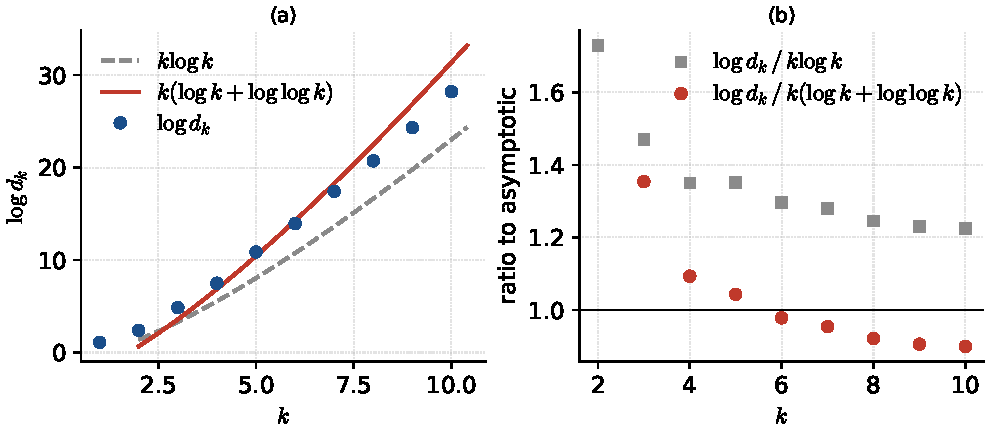
\includegraphics[width=0.94\textwidth]{fig_growth.pdf}
\caption{Growth of the staircase. (a)~$\log d_k$ (dots) against the leading
term $k\log k$ (dashed) and the refined leading behavior
$k(\log k+\log\log k)$ (solid). (b)~Ratios of $\log d_k$ to the two
asymptotic expressions; the second-order correction brings the ratio close
to $1$, and both converge to $1$ by Corollary~\ref{cor:main}(i).}
\label{fig:growth}
\end{figure}

\begin{figure}[htbp]
\centering
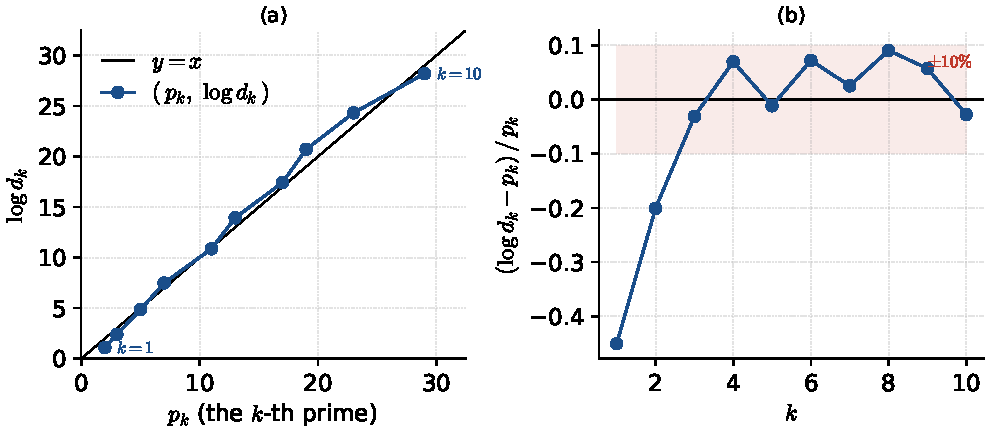
\includegraphics[width=0.94\textwidth]{fig_logd_pk.pdf}
\caption{The approximation $\log d_k\approx p_k$ of
Corollary~\ref{cor:main}(iii). (a)~The points $(p_k,\log d_k)$ for
$1\le k\le10$ against the line $y=x$. (b)~The relative error
$(\log d_k-p_k)/p_k$, which stays within $\pm10\%$ from $k=3$ onward.}
\label{fig:logdpk}
\end{figure}

The expansion of Corollary~\ref{cor:secondorder} converges rather slowly at
accessible values of $k$ --- the correction $(\log k)(1+\li(\log k))$ is
about $5.6$ at $k=10$, against an error term of size
$k(\log\log k)^2/\log k\approx3.0$ --- but its structure is fully confirmed
by the data: subtracting the main term
$k(\log k+\log\log k-1)$ and the correction $(\log k)(1+\li(\log k))$ from
$\log d_k$ leaves a remainder that decreases monotonically from $3.5$ at
$k=4$ to $1.2$ at $k=10$.

% =====================================================================
\section{Computability: how far can one climb?}\label{sec:computability}

By Proposition~\ref{prop:decomp}, computing $d_k$ exactly is the problem of
evaluating the $m_k$-th prime, where $m_k=f^{k}(k)$ is itself obtained by
$k$ nested evaluations of the $n$-th prime at arguments growing along the
orbit of $k$. The final step dominates the cost: by
Corollary~\ref{cor:main}, $d_k\approx e^{-1}k\log k\cdot m_k$, and a sieve
must essentially enumerate, or at least count, the primes up to
$d_k\approx(k\log k/e)^{k(1+o(1))}$. Since the terms of the index staircase
are known through $m_{14}$ (A058009; the last terms are due to D.~Johnson
and G.~Resta), the only obstacle to extending the staircase beyond $d_{10}$
is precisely this final prime evaluation.

All computations reported here were performed on two CPU cores with 4\,GB
of memory. The values $d_1,\ldots,d_7$ follow in milliseconds from nested
calls to \texttt{sympy.prime}. An odd-only segmented sieve of our own,
written in \texttt{numpy} with segments of $10^9$ integers, yields
$d_8=997\,525\,853$ in $3.5$ seconds and
$d_9=36\,294\,260\,117$ in about three minutes; its cumulative counts were
validated against the classical values $\pi(10^9)=50\,847\,534$,
$\pi(10^{10})=455\,052\,511$ and $\pi(10^{11})=4\,118\,054\,813$ crossed
during the run. Finally, compiling the \texttt{primesieve} library
\cite{primesieve} from source and evaluating the
$64\,988\,430\,769$-th prime gives
\[
  d_{10}=1\,765\,037\,224\,331
\]
in $3$ minutes $43$ seconds of wall time. Each value was cross-checked by
at least two independent implementations.

Beyond $d_{10}$, exact evaluation by sieving rapidly leaves the laptop
regime, but the indices are known, so rigorous brackets come almost for
free from the Dusert bounds $n(\log n+\log\log n-1)<p_n<n(\log n+\log\log
n)$ for $n\ge6$ \cite{Dusert}. Table~\ref{tab:bounds} lists them together
with the point estimates obtained by inverting $\li$ numerically at the
known indices --- an estimator whose accuracy is impressive: applied at
$m_{10}$ it predicts $1.765036\times10^{12}$ against the true value
$1.765037\times10^{12}$, a relative error below $10^{-5}$.

\begin{table}[htbp]
\centering
\small
\caption{The upper end of the computable range. Indices $m_k$ from A058009;
the brackets are the rigorous Dusert bounds for $d_k=p_{m_k}$; the estimates
invert $\li$ numerically. Digits refer to the estimates.}
\label{tab:bounds}
\begin{tabular}{@{}rrrrrr@{}}
\toprule
$k$ & index $m_k$ & lower bound & upper bound & estimate & digits\\
\midrule
11 & 2\,428\,095\,424\,619 & $7.495\times10^{13}$ & $7.738\times10^{13}$
  & $7.506\times10^{13}$ & 14\\
12 & 119\,543\,903\,707\,171 & $4.171\times10^{15}$ & $4.291\times10^{15}$
  & $4.177\times10^{15}$ & 16\\
13 & 5\,519\,908\,106\,212\,193 & $2.144\times10^{17}$ & $2.199\times10^{17}$
  & $2.146\times10^{17}$ & 18\\
14 & 248\,761\,474\,969\,923\,757 & $1.063\times10^{19}$ & $1.088\times10^{19}$
  & $1.064\times10^{19}$ & 20\\
\bottomrule
\end{tabular}
\end{table}

The cost ladder is now explicit. Sieving to $x$ costs on the order of
$x/\log x$ operations and $\mathcal{O}(\sqrt{x})$ memory, so
$d_{11}\approx7.5\times10^{13}$ is one to two core-hours away with a
well-optimized library such as \texttt{primesieve} --- an afternoon's
patience rather than a research problem. The step to
$d_{12}\approx4.2\times10^{15}$ is two orders of magnitude: days of
many-core sieving, at the limit of what is reasonable. For
$d_{13}\approx2.1\times10^{17}$ and $d_{14}\approx1.1\times10^{19}$,
sieving is hopeless, and the appropriate tool is analytic prime counting
(the Meissel--Lehmer--Lagarias--Miller--Odlyzko and
Del\'eglise--Rivat line of algorithms, as implemented in
\texttt{primecount} \cite{primesieve}), which evaluates $\pi(x)$, and hence
the $n$-th prime by bisection, in roughly $x^{2/3}$ operations and
$\mathcal{O}(x^{1/3})$ memory; at that scale $d_{13}$ and $d_{14}$ become
workstation computations of hours to days. Finally $d_{15}$ would first
require the index $m_{15}=p_{248\,761\,474\,969\,923\,757}$ itself, an
$n$-th prime at $n\approx2.5\times10^{17}$, and then the
$m_{15}$-th prime with $m_{15}\approx10^{21}$: two successive evaluations
at the frontier of current record computations. We therefore place the
practical horizon of exact evaluation at $k=14$, and note the convenient
rule of thumb, exact for $k\ge11$: \emph{the $k$-th staircase prime has
$2k-8$ decimal digits}.

% =====================================================================
\section{Concluding remarks and open problems}\label{sec:conclusions}

The prime staircase is arguably the most economical way of walking through
the hierarchy of higher-order primes: one index, one level per step. The
results of this note show that despite its superexponential growth it is
fully accessible to classical asymptotic analysis, and that its growth law
has a memorable avatar: $\log d_k$ is asymptotic to the $k$-th prime
itself.

We close with several problems.

\begin{proposition}\label{prop:counting}
Let $D(x)=\#\{k\ge1: d_k\le x\}$. Then
\[
  D(x)\sim\frac{\log x}{\log\log x}\qquad(x\to\infty).
\]
\end{proposition}

\begin{proof}
By Remark~\ref{rem:mk}, $m_k<d_k\le m_k^{1+\varepsilon}$ for every
$\varepsilon>0$ and all large $k$. Hence, with
$M(x)=\#\{k: m_k\le x\}$, for large $x$,
\[
  M\bigl(x^{1/(1+\varepsilon)}\bigr)\le D(x)\le M(x).
\]
Miska, T\'oth and \.Zmija proved $M(x)\sim\log x/\log\log x$
\cite[Theorem~12]{MiskaTothZmija}; applying this to both bounds and letting
$\varepsilon\to0$ gives the claim.
\end{proof}

\begin{enumerate}[leftmargin=1.6em,itemsep=2pt,topsep=4pt]
\item \emph{Complete asymptotic expansion.} The proof of
Theorem~\ref{thm:master} strongly suggests that $\log d_k$ admits a full
Cipolla-type expansion
$\sum_{i\ge0} c_i\,k\,P_i(\log k,\log\log k)$, and similarly for $m_k$;
already the correction $(\log k)(1+\li(\log k))$ of
Corollary~\ref{cor:secondorder} mixes the two scales $\log k$ and
$\log^2k/\log\log k$ in a way that a pure power series in $1/\log k$ cannot
capture. Making this precise, and controlling the sign of the remainder,
is open.
\item \emph{Arithmetic structure.} The staircase primes show no visible
congruence pattern: modulo $12$ their residues are
$3,11,7,7,11,1,5,1,5,1$ for $k=1,\ldots,10$. Do the staircase primes
equidistribute among the admissible residue classes in the (weak) sense of
natural density along the sequence?
\item \emph{Variants.} Every arithmetic self-map of $\N$ with image a
proper subset has a hierarchy and a staircase. The composite analogue,
based on iterating $n\mapsto c_n$ (the $n$-th composite,
\href{https://oeis.org/A280327}{A280327}), and the primeth-recurrence
crossings of the type in Proposition~\ref{prop:crossing} deserve study; so
does the iteration-count variant A344946, which meets the staircase at
$k=1,2$ and then diverges.
\item \emph{Cataloguing.} The sequence
\[
  3,\ 11,\ 127,\ 1787,\ 52711,\ 1128889,\ 37139213,\ 997525853,\
  36294260117,\ 1765037224331,
\]
with the brackets of Table~\ref{tab:bounds} beyond, is
proposed for inclusion in the OEIS.
\end{enumerate}

\subsection*{Acknowledgments}
The author thanks his friend, Albert Zotkin, whose questions about iterating the selection
of prime-indexed primes prompted this note.

% =====================================================================
\begin{thebibliography}{13}\small

\bibitem{Batchko}
R.~G. Batchko,
\href{https://arxiv.org/abs/1405.2900}{A prime fractal and global
quasi-self-similar structure in the distribution of prime-indexed primes},
arXiv:1405.2900 [math.GM], 2014.

\bibitem{Bayless}
J. Bayless, D. Klyve, and T. Oliveira e Silva,
\href{http://integers-ejcnt.org/n43/n43.Abstract.html}{New bounds and
computations on prime-indexed primes}, Integers \textbf{13} (2013),
\#A43.

\bibitem{BroughanBarnett}
K.~A. Broughan and A.~R. Barnett,
\href{https://cs.uwaterloo.ca/journals/JIS/VOL12/Broughan/broughan16.html}{On
the subsequence of primes having prime subscripts}, J. Integer Seq.
\textbf{12} (2009), Article 09.2.3.

\bibitem{Cipolla}
M. Cipolla,
La determinazione asintotica dell'$n$-mo numero primo (in Italian),
Rend. Accad. Sci. Fis. Mat. Napoli (3) \textbf{9} (1903), 132--166.

\bibitem{DresslerParker}
R.~E. Dressler and S. Parker,
\href{https://doi.org/10.1145/321892.321900}{Primes with a prime
subscript}, J. ACM \textbf{22} (1975), no.~3, 380--381.

\bibitem{Dusert}
P. Dusart,
\href{https://arxiv.org/abs/1002.0442}{Estimates of some functions over
primes without R.H.}, arXiv:1002.0442 [math.NT], 2010.

\bibitem{Fernandez}
N. Fernandez,
\href{http://www.borve.org/primeness/FOP.html}{An order of primeness,
$F(p)$}, 1999.

\bibitem{GutmanIvic}
I. Gutman and A. Ivi\'c,
\href{https://doi.org/10.1016/0012-365X(95)00182-V}{On Matula numbers},
Discrete Math. \textbf{150} (1996), no.~1--3, 131--142.

\bibitem{MiskaTothZmija}
P. Miska, J.~T. T\'oth, and B. \.Zmija,
\href{https://arxiv.org/abs/1908.10421}{On distribution of subsequences of
primes having prime indices with respect to the $(R)$-denseness and
convergence exponent}, arXiv:1908.10421 [math.NT], 2019.

\bibitem{primesieve}
K. Walisch,
\href{https://github.com/kimwalisch/primesieve}{primesieve and primecount:
fast C/C++ prime number generators and counters}, software, 2026.

\bibitem{HigherOrderWiki}
OEIS Wiki,
\href{https://oeis.org/wiki/Higher-order_prime_numbers}{Higher-order prime
numbers}, OEIS Foundation.

\bibitem{OEIS}
N.~J.~A. Sloane (ed.),
\href{https://oeis.org}{The On-Line Encyclopedia of Integer Sequences},
OEIS Foundation Inc. Sequences
\href{https://oeis.org/A000040}{A000040},
\href{https://oeis.org/A006450}{A006450},
\href{https://oeis.org/A007097}{A007097},
\href{https://oeis.org/A038580}{A038580},
\href{https://oeis.org/A049090}{A049090},
\href{https://oeis.org/A049076}{A049076},
\href{https://oeis.org/A058009}{A058009},
\href{https://oeis.org/A354967}{A354967}.

\bibitem{RosserSchoenfeld}
J.~B. Rosser and L. Schoenfeld,
\href{https://doi.org/10.1215/ijm/1255631807}{Approximate formulas for some
functions of prime numbers}, Illinois J. Math. \textbf{6} (1962), no.~1,
64--94.

\end{thebibliography}

\end{document}
